% !TEX root = ../report.tex

\section{Stakeholders}
\label{sec:stakeholders}
This section presents the stakeholders and their concerns. The main concerns are listed in bold and, where applicable, the specific concern in parentheses. \\

Docker has the following stakeholders:
\begin{itemize}
	\item Software developers
	\item Software Maintainers
	\item Cloud providers
	\item The open container initiative
	\item Docker developers
	\item Plugin developers
\end{itemize}

%\item [Product owner] is the owner of the system. This stakeholder funds the project.  This affects the quality attributes usability and availability.
\subsection*{Software Developers}
The developers are those that use Docker to create their software systems. Docker is used by developers to deploy software and create architectures consisting of multiple containers. Developers using Docker for their system, expect it to work according to the documentation and have a good usability.
%TODO source

\textbf{Concerns}
\begin{description}[labelwidth=6cm,labelindent=30pt,style=multiline,leftmargin=5.5cm,font=\normalfont\itshape]

% Usuability
%		- Appropriateness recognizability. Degree to which users can recognize whether a product or system is appropriate for their needs.
%		- Learnability. degree to which a product or system can be used by specified users to achieve specified goals of learning to use the product or system with effectiveness, efficiency, freedom from risk and satisfaction in a specified context of use.
%		- Operability. Degree to which a product or system has attributes that make it easy to operate and control.
%User error protection. Degree to which a system protects users against making errors.
%		- User interface aesthetics. Degree to which a user interface enables pleasing and satisfying interaction for the user.
%		- Accessibility. Degree to which a product or system can be used by people with the widest range of characteristics and capabilities to achieve a specified goal in a specified context of use.

%Reliability
%		- Maturity. Degree to which a system, product or component meets needs for reliability under normal operation.
%		- Availability. Degree to which a system, product or component is operational and accessible when required for use.
%		- Fault tolerance. Degree to which a system, product or component operates as intended despite the presence of hardware or software faults.
%		- Recoverability. Degree to which, in the event of an interruption or a failure, a product or system can recover the data directly affected and re-establish the desired state of the system.

%Portability
%Adaptability. Degree to which a product or system can effectively and efficiently be adapted for different or evolving hardware, software or other operational or usage environments.
%Installability. Degree of effectiveness and efficiency with which a product or system can be successfully installed and/or uninstalled in a specified environment.
%Replaceability. Degree to which a product can replace another specified software product for the same purpose in the same environment.

\item[\textbf{Usability}] Since the software developers are using Docker, they want it to have good usability. This means it is easy to learn how to use Docker and it is not hard to work with. In fact, this is one of the main benefits of Docker, since it makes it easier to containerize applications, which could be done before, but was very difficult to do in practice.


\item[\textbf{Functional Suitability} (Functional correctness)] Software developers care about the functional correctness, since bugs in the Docker software make the development of their software more difficult. 

\end{description}

\subsection*{Software Maintainers}
Software maintainers are responsible for deploying the software and keeping the software product running. Docker is often used for software deployment (especially to the cloud). %TODO source
The software maintainers expect Docker to be reliable, portable, efficient and secure.

\textbf{Concerns}
\begin{description}

%[labelindent=25pt,style=multiline,leftmargin=4.0cm,font=\normalfont\itshape]

\item[\textbf{Reliability}] Software maintainers are responsible for keeping the software working while it is deployed. They will only use Docker if it is reliable. It has to be tolerant against failing containers.

\item[\textbf{Portability}] The software maintainers want to be able to run Docker and its containers on a variety of different environments.

\item[\textbf{Performance efficiency}] The software maintainers want Docker to have a good performance. They want the resources of their servers to be used as efficiently as possible and therefore want Docker to have almost no overhead, like Virtual Machines often do have.


\item[\textbf{Security}] Software maintainers want Docker to be secure, so applications can be run inside the containers, without Docker negatively affecting the security of this application.


\end{description}



\subsection*{Cloud providers}
There are numerous cloud providers offering services which are based on Docker\footnote{\url{https://www.docker.com/partners\#/service}}. These cloud providers offer Container-based cloud computing, sometimes referred to as CaaS (Containers-as-a-Service).


\textbf{Concerns}
\begin{description}[labelindent=25pt,style=multiline,leftmargin=4.0cm,font=\normalfont\itshape]

\item[\textbf{Portability} (Installability)] The cloud providers want to integrate Docker into their cloud computing architecture.\\ 

\item[\textbf{Compatibility} (Co-Existence)] Docker has to share the environment with the existing architecture of the cloud providers.

\item[\textbf{Reliability}] The customers using the cloud providers' services expect a high reliability. If cloud providers are to implement Docker in their architectures, they need Docker to be as reliable as running the application naively or inside a VM.

\item[\textbf{Security}] Cloud providers want to offer a secure cloud computing environment to their customers.
\end{description}



\subsection*{The Open Container Initiative}

The Open Container Initiative\footnote{\url{https://www.opencontainers.org/}} was formed with the purpose of creating an open industry standard for container formats and runtime in June 2015.

They are interested in creating a formal, open, industry specification around container formats and runtime. This specification should be independent of particular clients/orchestration stacks, commercial vendors or projects and should be portable across a wide variety of operating systems, hardware etc.
% ^ according to about page

Docker has donated its container format and runtime, known as `runC' to this initiative and is one of the members of the initiative, together with a lot of other members (including competing technologies, such as `rkt' from CoreOS)\footnote{A list is available at \url{https://www.opencontainers.org/about/members}}.

\textbf{Concerns}
\begin{description}[labelindent=25pt,style=multiline,leftmargin=4.0cm,font=\normalfont\itshape]

\item[\textbf{Portability}] The main goal of the initiative is to standardize the format for the container and the runtime. These standards are used by Docker to allow using Docker containers with other container runtimes.

\item[\textbf{Compatibility} (Interoperability)] Docker has to be able to work with the containers from the initiative.

\end{description}

\subsection*{Docker developers}
The Docker developers are the developers contributing to the Docker code base. Some of these developers work on Docker in their free time, others work on it as part of their job at a company with an interest in Docker and some developers work for Docker Inc itself\cite{whoaredockerdevs}.

\textbf{Concerns}
\begin{description}[labelindent=25pt,style=multiline,leftmargin=4.0cm,font=\normalfont\itshape]

\item[\textbf{Maintainability} \textit{(Modifiability)}] These developers contribute new features and bugfixes to the existing code base. Therefore, they want the project to have good modifiability, such that additions and improvements can be realized without to much effort.

%\item[Functional correctness]
\item[\textbf{Security}] The Docker developers care about the security of the product they are working on.\footnote{\url{https://github.com/docker/docker\#security-disclosure}}  % somebody has to care about it


\end{description}

\subsection*{Plugin developers}
Docker allows extending its capabilities with plugins\footnote{\url{https://blog.docker.com/2015/06/extending-docker-with-plugins/}}. These plugins are created by the plugin developers.

\textbf{Concerns}
\begin{description}[labelindent=25pt,style=multiline,leftmargin=4.0cm,font=\normalfont\itshape]

\item[\textbf{Portability} (Adaptability)] The developers of the plugins want to extend the functionality of Docker in an effective and efficient way. 

\end{description}

\subsection*{Overview}
The stakeholders and their related concerns are visualized in Figure~\ref{fig:stakeholders-quality} below.

\begin{figure}[H]
\centering
%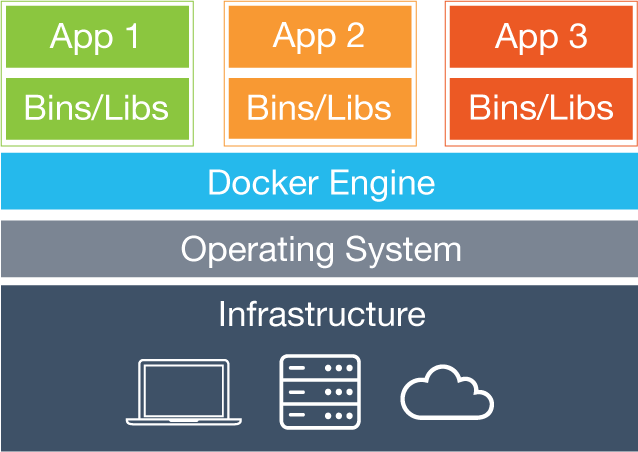
\includegraphics[scale=0.4]{5-patterns/images/what-is-vm-diagram.png}
% \paperwidth
\begin{center}
  \makebox[\textwidth]{
	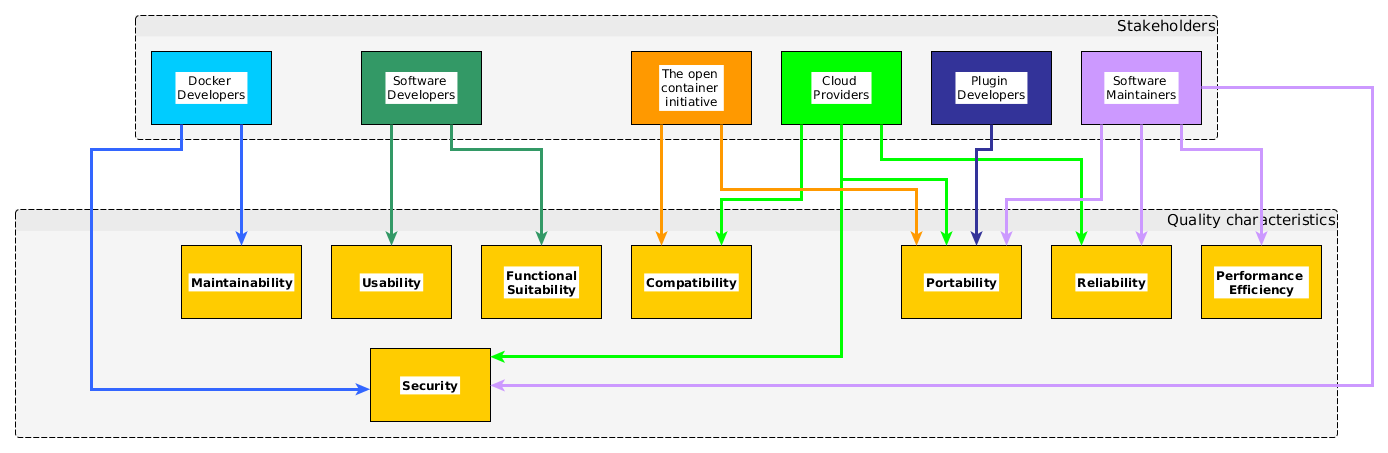
\includegraphics[width=0.9\paperwidth]{3-stakeholders/images/StakeholderQuality.png}}
\end{center}
\caption{Stakeholders and the quality attributes they are concerned about}
\label{fig:stakeholders-quality}
\end{figure}



%
%\begin{table}[H] \centering
%	\caption{Matrix of stakeholders concern.}
%	\label{table:stakeholder_concern}
%	\begin{tabular}{@{} cl*{10}c @{}}
%		&  & \multicolumn{8}{c}{
%		\textbf{Concerns}} \\[2ex]
%		& \textbf{Stakeholder} 
%			& 
%			& \rot{Functional suitability}
%			& \rot{Performance efficiency}
%			& \rot{Compatibility}
%			& \rot{Usability}
%			& \rot{Reliability}
%			& \rot{Security}
%			& \rot{Maintainability}
%			& \rot{Portability}			
%			\\
%		\midrule
%								%ada	co-ex	impl	maint	perfor	port	relia	usa	
%& Software developer 	& &		&		&		&		&		&		&		X&		X 		\\
%& Software main 		& &		&		&		&		&		X&		X&		X&				\\				
%& Cloud providers 		& &		&		X&		X&		&		&		&		X&				\\			
%& The open container 
%initiative 				& &		&		&		&		&		&		X&		&				\\	
%& Docker developers 
%						& &		&		&		&		X&		&		&		&				\\				
%& Plugin developers 
%						& &		X&		&		&		&		&		&		&				\\				
%\midrule
%& Total					& &		1&	   1&	    1& 		1& 		1&		2&		3&		1		\\
%\midrule
%	\end{tabular}
%\end{table}
